\chapter{生命的各个阶段}\label{ch:g3:stages-of-life}

想象一张全家福：婴儿坐在奶奶的膝上，
缺了两颗门牙的小学生，突然长高的青少年表哥，
比他妈妈还高，还有父母和奶奶本人。一家人，
一个下午——整个人类\omterm{def:g2:born-grow-die:cycle}{生命周期}就坐在
一张沙发上。本章将仔细观察这些阶段，以及
生长本身如何被测量。

\section{人的一生的各个阶段}

\begin{definition}[人的生命阶段]\label{def:g3:stages-of-life:stages}
人的一生会经历若干阶段：
\begin{enumerate}
  \item \emph{婴儿}\index{婴儿}（大约出生后的前两
        年）：生长最快，长出第一颗牙，迈出第一步，
        说出第一个词；
  \item \emph{儿童}\index{儿童}：稳定生长，\omterm{prop:g2:teeth-and-eating-well:sets}{乳牙}
        逐渐换成\omterm{prop:g2:teeth-and-eating-well:sets}{恒牙}，学习各种本领；
  \item \emph{青少年}\index{青少年}：
        出现又一次快速生长，身体
        由儿童逐渐变为成人；
  \item \emph{成体}\index{成体}：身高不再增长；
        可以为人父母；
  \item \emph{老年期}\index{老年期}：头发变白，\omterm{def:g1:the-five-senses:sense}{皮肤}
        起皱纹，力气慢慢减弱——这是
        \omterm{def:g2:born-grow-die:cycle}{生命周期}中自然的最后阶段。
\end{enumerate}
\end{definition}

\begin{example}[读懂沙发上的一家人]\label{ex:g3:stages-of-life:sofa}
在家人的沙发上：婴儿（阶段 1），
缺门牙的小学生（阶段 2——换牙正值高峰，
参见\cref{ch:g2:teeth-and-eating-well}），
十六岁的表哥（阶段 3，快速生长正在中途），父母（阶段
4），奶奶（阶段 5）。五个阶段，一家人。
\end{example}

\begin{omfigure}
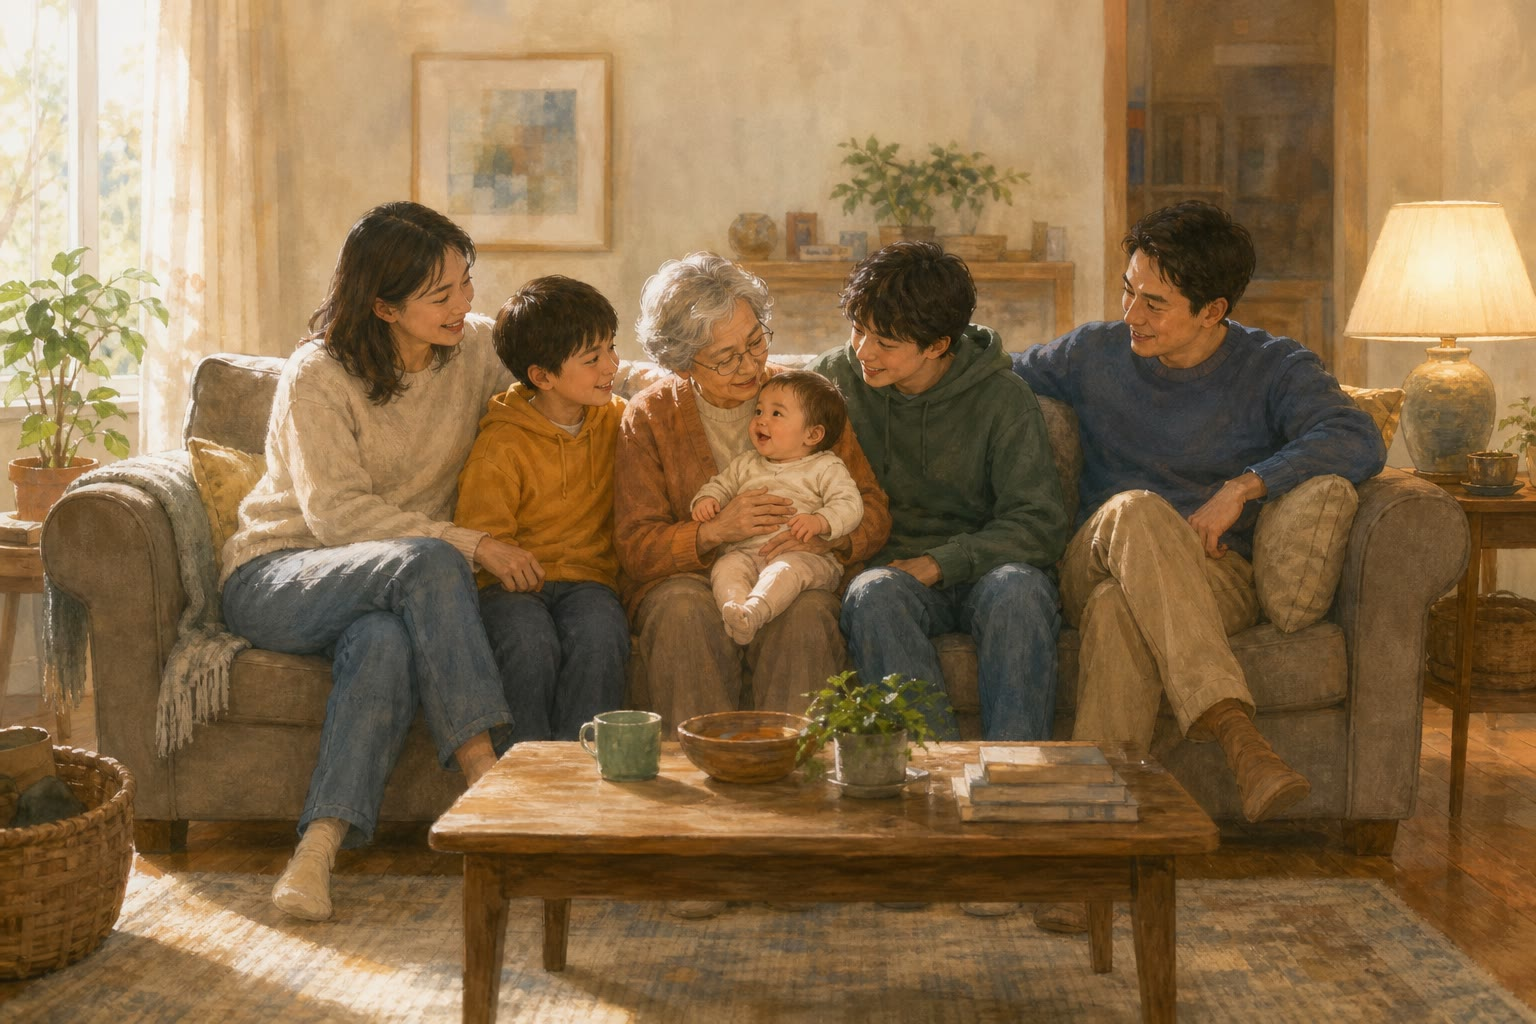
\includegraphics[width=0.62\linewidth]{images/book1/ai/g3-stages-family.jpg}

{\small 整个\omterm{def:g2:born-grow-die:cycle}{生命周期}坐在一张沙发上：婴儿、儿童、青少年、
\omterm{def:g3:stages-of-life:stages}{成体}、奶奶。}
\end{omfigure}

\begin{remark}[生长并不均匀]\label{rem:g3:stages-of-life:bursts}
生长有节奏：婴儿期最快——第一年身高
约增加一半；童年期生长较慢且稳定，
青少年期再次加快，之后便停止。两次
快速生长中间夹着一段平稳期：这就是
正常的成长模式。
\end{remark}

\section{测量生长}

\begin{definition}[生长曲线图]\label{def:g3:stages-of-life:chart}
\emph{生长曲线图}\index{生长曲线图}是对身高
（或体重）随时间反复测量所得的记录，
就像\cref{ch:g1:my-body}中的门框刻度，只是更规整并标注了日期。
医生会为每个儿童保存一份。
\end{definition}

\begin{omfigure}
\begin{tikzpicture}
\begin{axis}[omaxis,
    width=9.2cm, height=6cm,
    xlabel={年龄（岁）}, ylabel={身高（厘米）},
    xmin=0, xmax=22.5, ymin=0, ymax=190,
    xtick={0,5,10,15,20},
    ytick={50,100,150},
    ]
  \addplot[very thick, omDef, smooth] coordinates {
    (0,50) (1,75) (2,87) (4,102) (6,115) (8,127) (10,138)
    (12,150) (14,165) (16,175) (18,178) (20,178)
  };
\end{axis}
\end{tikzpicture}

{\small 从出生到成年的\omterm{def:g3:stages-of-life:chart}{生长曲线图}：婴儿期
曲线陡峭，儿童期平缓，青少年期再次陡峭，
之后平缓——生长结束。}
\end{omfigure}

\begin{example}[读懂曲线图]\label{ex:g3:stages-of-life:reading}
在曲线图上，线条在最初的一年内约上升 $\qty{25}{cm}$，
而在童年期每年仅约上升 $\qty{6}{cm}$ 。
两段陡峭部分对应
\cref{rem:g3:stages-of-life:bursts}中的两次快速生长；平坦的末端说明
成年人已经不再长高。
\end{example}

\begin{method}[记录你自己的生长曲线]\label{met:g3:stages-of-life:keep}
\begin{enumerate}
  \item 认真测量身高（用墙壁和书本的方法，
        就是之前学过的方法），测量时始终不穿鞋；
  \item 在笔记本上写下日期和身高，或在
        门框上做记号并标注日期；
  \item 每隔几个月再测一次——坚持规律比
        频率更重要；
  \item 要看清变化过程，把数据点画出来：年龄沿下方，
        身高沿竖直方向，与图中一样。
\end{enumerate}
\end{method}

\section{动物和植物也有各个阶段}

\begin{proposition}[生物界中的各个阶段]\label{prop:g3:stages-of-life:animals}
每种\omterm{def:g1:living-or-not:living}{生物}都会经历其自身版本的\omterm{def:g2:born-grow-die:cycle}{生命周期}：
幼体、\omterm{def:g3:stages-of-life:stages}{成体}和\omterm{def:g3:stages-of-life:stages}{老年期}。幼体阶段可能
与\omterm{def:g3:stages-of-life:stages}{成体}相似（如小猫、小马驹），或完全不同（如
\omterm{ex:g2:animals-grow-up:frog}{蝌蚪}，或\cref{ch:g2:animals-grow-up}中的\omterm{ex:g2:animals-grow-up:butterfly}{毛毛虫}）；
\omterm{def:g1:plants-around-us:plant}{植物}的阶段依次为\omterm{def:g2:from-seed-to-plant:seed}{种子}、\omterm{prop:g2:from-seed-to-plant:cycle}{幼苗}、幼株、开花的\omterm{def:g3:stages-of-life:stages}{成体}。
任何\omterm{def:g1:living-or-not:living}{生物}都不能跳过阶段，也不能倒过来经历。
\end{proposition}
\admitted

\begin{example}[快与慢]\label{ex:g3:stages-of-life:speeds}
不同\omterm{def:g1:living-or-not:living}{生物}的速度相差极大。苍蝇几周就成年；猫
大约一年成年；人将近二十年才成年；橡树
要经过几十年才长出第一批橡子。无论快慢，
阶段的顺序都不会改变。
\end{example}

\begin{remark}[老年是一个阶段，而非缺陷]\label{rem:g3:stages-of-life:oldage}
白发和皱纹并不是疾病，它们是身体的
最后一个阶段，和婴儿长出第一颗牙一样自然。在许多
物种中，包括人类家庭里，年长者拥有
年轻人最需要的东西——经验。
\end{remark}

\section{练习}

\begin{exercise}[$\star$]\label{exo:g3:stages-of-life:1}
按顺序写出人一生的五个阶段。
\end{exercise}

\begin{exercise}[$\star$]\label{exo:g3:stages-of-life:2}
在哪个阶段：(a) \omterm{prop:g2:teeth-and-eating-well:sets}{乳牙}会脱落？
(b) 人能否成为父母？(c) 生长在整个一生中是否最快？
\end{exercise}

\begin{exercise}[$\star$]\label{exo:g3:stages-of-life:3}
生长的两次高峰是什么？它们之间处于哪个阶段？
\end{exercise}

\begin{exercise}[$\star$]\label{exo:g3:stages-of-life:4}
在\omterm{def:g3:stages-of-life:chart}{生长曲线图}上，仅凭曲线本身，
如何判断成年人已经停止生长？
\end{exercise}

\begin{exercise}[$\star$]\label{exo:g3:stages-of-life:5}
利用曲线图，估计在 $6$ 岁到 $8$ 岁之间，
曲线大约上升了多少厘米？第一年呢？
\end{exercise}

\begin{exercise}[$\star$]\label{exo:g3:stages-of-life:6}
为什么身高每次都必须在不穿鞋的情况下、以相同的方式测量？
如果不这样，可能会出现什么问题？
\end{exercise}

\begin{exercise}[$\star$]\label{exo:g3:stages-of-life:7}
写出橡树从橡子到老树的各个生命阶段。
\end{exercise}

\begin{exercise}[$\star$]\label{exo:g3:stages-of-life:8}
试一试：为你自己开始绘制
\cref{met:g3:stages-of-life:keep}中的\omterm{def:g3:stages-of-life:chart}{生长曲线图}，记录今天的第一个数据点。
你目前处于\cref{def:g3:stages-of-life:stages}中的哪个阶段？
还有哪一次生长高峰尚未到来？
\end{exercise}

\begin{exercise}[$\star\star$]\label{exo:g3:stages-of-life:9}
苍蝇、猫、人和橡树经历相同的阶段，
但速度差异很大。请将它们按达到成年所需时间
从快到慢排序，并说明这四种阶段顺序
有什么共同之处。
\end{exercise}

\begin{exercise}[$\star\star$]\label{exo:g3:stages-of-life:10}
汤姆今年 $9$ 岁，一个月内两次测量自己的身高，
发现“完全没有长高”。他需要担心吗？请结合
\cref{rem:g3:stages-of-life:bursts}和他这个年龄段的
曲线形状来回答。
\end{exercise}
